\chapter{Black Hole at the Galactic Center?}

\section{Mystery at the Center of the Milky Way}
\begin{steps}
	\item Take a moment to watch the video found in the following link \url{www.astro.ucla.edu/~ghezgroup/gc/animations.html} under the heading \textbf{3D Movie of Stellar Orbits in the Central Parsec}.
\end{steps}
At first glance the video might not seem all too surprising as having learned about the solar system you likely expect orbiting planets to be a mundane fixture of the universe. However, what if you were to learn that the objects were not planets, but in fact stars and that what you see in the video spans a distance of 3 light years? For comparison, Pluto is only about $0.0006\:$ly from the sun. In fact, the video you just saw is a visualization of a phenomenon in the center of our galaxy which puzzled astronomers for a long time. As you might have learned all objects exert a gravitational force which is proportional to the mass of the object. For this reason, smaller objects tend to be ``pulled in'' by larger objects, forming the orbital relationships we see in our daily lives: the moon orbiting the Earth, the Earth orbiting the Sun, and so on. Some of the most massive objects in the universe are stars which is why they tend to form the center of orbital systems. However, given that all the objects in the video were stars, this meant that there had to be a much, much more massive object in the center of our galaxy attracting them, one which seemed to be invisible, save for radio signals coming from the location of the object. There were many theories as to what the object, whose signal is dubbed Sagittarius A*, could  be. Some believed it to be a collection of massive objects such as stars or small black holes. The most compelling theory, however, was that thee source responsible for the signal was, in fact, a Supermassive Black Hole (SMBH).
Black holes are some of the most extreme objects in the universe which were first theorized to exist as a result of Einstein's theory of general relativity. In the most basic terms, a black hole is an extremely massive and dense object whose gravitational pull is so strong, that not even light can escape. This fact that light cannot escape from a black hole,  however, makes them incredibly difficult to observe directly. That said, due to the strength of their gravitational pull, black holes can often be detected indirectly based on their influence over nearby objects.

In this lab you will examine the gravitational system you saw in the video and see what judgment you can make about whether the object in the center of the Milky Way is, in fact, a black hole.% First, however, you will learn about the basic laws which govern orbital systems and how they can be applied to determine some of the physical properties of the objects in the system.

\section{Learning Goals}
\begin{itemize}
	\item Understand Kepler's laws of planetary motion and be able to use them to extract information about orbital systems.
	\item Be able to gather data using a variety of tools and understand the limitations of experimental data.
	\item Be able to make inferences about physical properties of objects which cannot be directly measured.
	\item Identify assumptions made during analysis and their effects on calculations.
\end{itemize}

\section{Team roles}

\begin{steps}
	\item \textbf{Decide on roles} for each group member.
\end{steps}

The available roles are:

\begin{itemize}
	\item Facilitator: ensures time and group focus are efficiently used
	\item Scribe: ensures work is recorded
	\item Technician: oversees apparatus assembly, usage
	\item Skeptic: ensures group is questioning itself
\end{itemize}

These roles can rotate each lab, and you will report at the end of the lab report on how it went for each role. If you have fewer than 4 people in your group, then some members will be holding more than one role. For example, you could have the skeptic double with another role. Consider taking on a role you are less comfortable with, to gain experience and more comfort in that role.

Additionally, if you are finding the lab roles more restrictive than helpful, you can decide to co-hold some or all roles, or think of them more like functions that every team needs to carry out, and then reflecting on how the team executed each function.

\section{Add members to Canvas lab report assignment group}

\begin{steps}
	\item On Canvas, navigate to the People section, then to the ``Lab 4 Groups'' tab. Find a group that is not yet used, and have each person in your group add themselves to that same lab group.
\end{steps}

This enables group grading of your lab report. Only one person will submit the group report, and all members of the group will receive the grade and have access to view the graded assignment.

\section{Installing ``ImageJ''}
For some parts of this lab you will be using a image analysis software called ``ImageJ'' to gather numerical data from images.
\begin{steps}
	\item Go to the following link to install the imageJ software \url{https://imagej.nih.gov/ij/download.html}
	\item Click on the link to the software version for your OS. This will download a .zip file.
	\item Once the file is downloaded, right click on the folder and choose ``extract all''. Once it is finished go into the folder you extracted the files to and click on the icon labeled ``Imagej''
\end{steps}

\section{Testing experiment: Is Sag A* a black hole?}

\subsection{Goal}

Test the hypothesis that Sag A* is a black hole by measuring the mass, determining it's Schwarzchild radius, measuring its maximum radius, and then comparing those radii.

\subsubsection{Equipment}
\begin{itemize}
	\item ImageJ: \url{https://imagej.nih.gov/ij/download.html}. This is an image processing program which you will use this to extract numerical data from the video
	\item Stars Orbiting Galactic Center: \url{https://youtu.be/7vcSKbXnLJA}. This is the video you will be analyzing
\end{itemize}

\subsection{General Relativity and Schwarzschild Radii}
While Newtonian dynamics is useful for describing most orbital systems, extreme systems or objects such as black holes cannot be fully described without also incorporating general relativity. In particular for this lab we will be using a particular description of the universe in which gravity, rather than being an ``attraction'' between objects, is actually the result of curved ``spacetime''. To visualize this, imagine space-time as sheet of stretched out fabric. Normally, if you were to try to roll light objects across the sheet they would travel in a straight line. However, if you were to place a large weight in the center, the fabric would droop inwards and any object you tried to roll would instead fall inwards towards the depressed region (the following video demonstrates this analogy: \url{https://youtu.be/MTY1Kje0yLg}). This is analogous to the effect that gravity has on spacetime. The key to this description is that anything traveling through spacetime will follow this curvature, even if it has no mass such as light. This means that, theoretically, an object can exist which bends spacetime so much that not even light can climb back out and escape (it would orbit the object or fall back inward). Using the principles of gravitation developed by Newton, we can estimate how massive and small such an object would be.

In Newtonian dynamics, the minimum speed an object needs to escape the gravitational pull of an object is given by 
\begin{equation}\label{gc:eq:escape-speed}
v_\textrm{escape} = \sqrt{\frac{2 G M}{r}} \,.
\end{equation}
where $r$ is the distance from its center of mass $M$.

\begin{steps}
	\item  First, manipulate this equation in order to get an expression for $r$ in terms of the other variables.
\end{steps}
If you now plug in the speed of light $c = 2.998 \times 10^{8}\:$m/s as the escape velocity into the equation you just derived, you get an expression for what is known as the Schwarszchild radius. The Schwarzschild radius is an estimate of the upper limit of the radius of a black hole with a given mass. That is, according to this model, if a chunk of matter of mass $M$ is squeezed into a radius as small or smaller than the radius $r$, then light cannot escape, and it is a black hole.

\begin{steps}
	\item To gain some intuition about how compact black holes would need to be, calculate the Schwarzchild radius for each of the following objects, and compare them to their actual radii.
	\begin{enumerate}
		\item One of your group members.
		\item the Earth.
		\item the Sun.
		\item the Solar System.
		\item The Milky Way Galaxy.
	\end{enumerate}
\end{steps}

To determine whether the object at the center of our galaxy is a black hole, we need to measure its mass, calculate its Schwarzchild radius based on that, then measure its radius and compare them.

\subsection{Finding the mass of Sag A* using stellar orbits}

%todo INTRO TEXT

In general, an \textit{orbit} is what we call the path an object follows when under the gravitational influence of a larger mass. The interactions between two gravitationally bound objects can be approximated using Newtonian mechanics, with the force of gravity between two objects given by 
\begin{equation}\label{gc:eq:newton}
F_\textrm{grav} = G \frac{m_1 \: m_2}{r^2} \, ,
\end{equation}
where $m_1$ and $m_2$ are the masses of the two objects, $r$ is the distance between them, and $G$ is the Newtonian constant of gravitation, $G=6.67 \times 10^{-11}\:\textrm{m}^3 \: \textrm{kg}^{-1} \: \textrm{s}^{-2}$. This equation, coupled with Newton's Second Law of Motion $F = ma$ or force $F$ equals mass $m$ times acceleration $a$, tells us that the stronger the force of gravity, the greater the acceleration due to gravity. With these two fundamental principles, it is possible to derive many of the properties of orbital mechanics. Moreover, they allow us to understand the physics behind the mathematical description of orbits formulated by Johannes Kepler nearly a century earlier.

\subsubsection{Orbits, ellipses, and Kepler's First Law}
Kepler's First Law states that \textit{a planet orbits the Sun in an ellipse, with the Sun at one focus of the ellipse}. This is true generally for any mass orbiting a much more massive object. An \textit{ellipse} (commonly referred to as an oval) is a generalization of a circle, allowing for the circle to be stretched along a certain direction. See Figure~\ref{gc:fig:ellipse} for details.

\begin{figure}
	\centering
	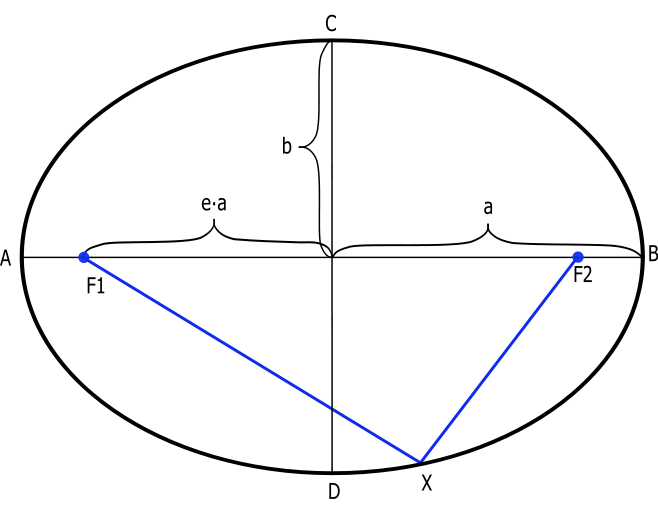
\includegraphics[width=0.6\textwidth]{galactic-center/ellipse.png}
	\caption{The geometry of an ellipse: $a$ is the semi-major axis of the ellipse, F1 and F2 are each a
		focus of the ellipse, $b$ is the semi-minor axis, and $e$ is the eccentricity. The eccentricity describes
		the extent to which the ellipse is oblong: an ellipse with $e = 0$ is just a circle. The foci are defined such
		that the distance from F1 to X, added to the distance from F2 to X, is the same no matter where X
		is located on the ellipse. For a circle, the foci coincide at the center. The Newtonian generalization of
		Kepler's First Law tells us that a small mass will orbit a much larger mass on an ellipse, and the larger
		mass will be located at one of the foci.}\label{gc:fig:ellipse}
\end{figure}

\subsubsection{Kepler's Third Law}

Kepler’s Third law addresses the path of an object $m$ as it orbits a much more massive object of mass $M$. Specifically, it relates the orbital period $P$ (the time it takes for one complete orbit to occur) to the semi-major axis $a$ of the ellipse according to
\begin{equation}\label{gc:eq:kepler-3}
P^2 = \frac{4 \pi^2}{G M} a^3 \,,
\end{equation}
where other objects are also considered to be not affecting the orbit of $m$. %\textbf{This is the
%	equation you will be using later to find the mass of Sag A*.}

An important qualification to be made about Kepler’s Laws is that they apply only to two-body
systems. Kepler’s third law breaks down when you have more than 2 orbiting objects in a system.
However, they are nonetheless a very good approximation for the orbits of small masses around a much
larger mass, in which case the gravitational force of the massive object dominates over the intra-small-
object interactions, and thus each smaller body approximately behaves independently from the other
small objects. And so the motion of each small object, to a good approximation, can be modeled by
Kepler’s laws.

\section{Developing Orbital Dynamics Skills}

%\subsubsection{Kepler's Second Law}
%The second law states that \textit{a line connecting a planet to the Sun sweeps out equal areas in
%equal time intervals}. This concept is demonstrated in Figure~\ref{gc:fig:keplers-2nd-ellipse}. As a consequence of this, when a
%planet is closer to the sun, it moves with a faster velocity. Furthermore, planets that have more circular
%orbits will have more uniform velocities over the course of their orbit than those with very eccentric
%orbits.
%
%\begin{figure}
%	\centering
%	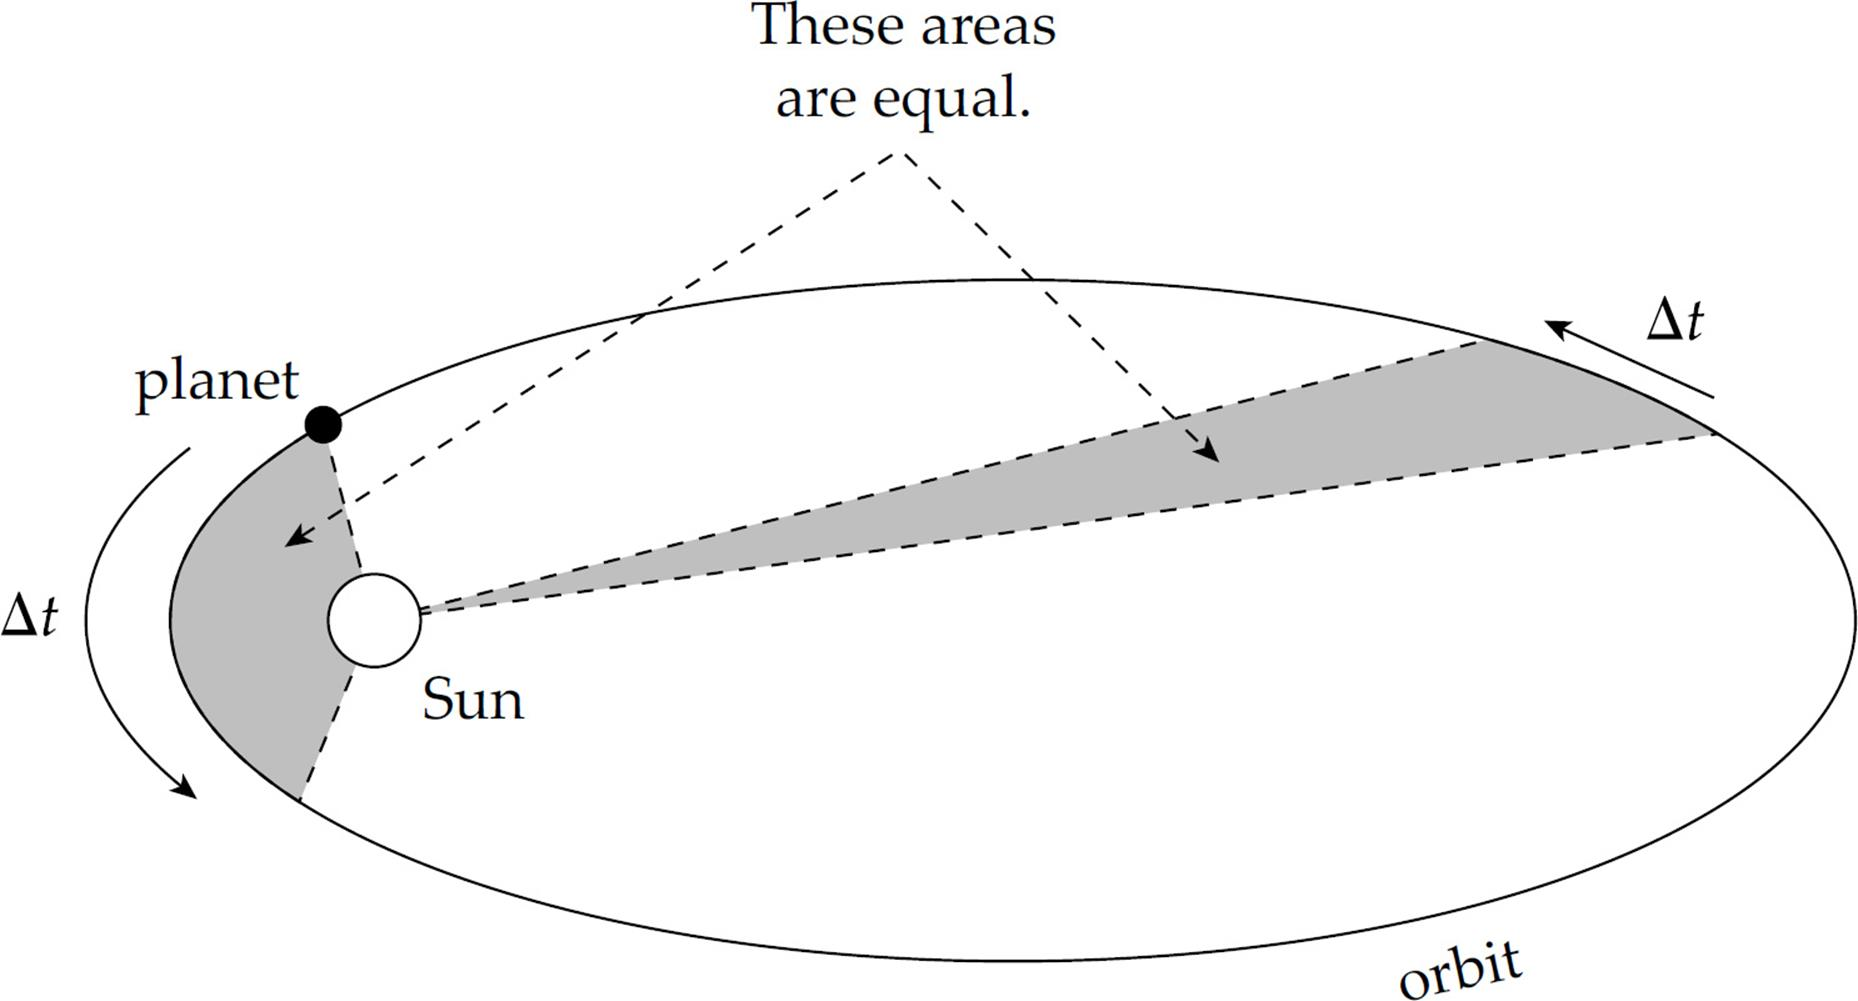
\includegraphics[width=0.7\textwidth]{galactic-center/keplers-2nd-ellipse.png}
%	\caption{Illustration of Kepler’s Second Law. The shaded regions are of equal area, so by Kepler’s Second Law, the
%		planet passes through each region of the orbit in the same amount of time. Since the region of the orbit
%		where the planet is closest to the Sun is a much further distance, and speed is change in position divided by
%		change in time, the planet will move with a much faster average speed than at the other portion of the
%		orbit, far away from the sun.}\label{gc:fig:keplers-2nd-ellipse}
%\end{figure}


\subsection{Goal}
Use Kepler's 3rd Law to analyze a test system.
\subsection{Available equipment}
\begin{itemize}
	\item Elliptical Orbits and Kepler's Laws simulator: \url{https://ophysics.com/f6.html}
\end{itemize}

\subsection{Steps}
\begin{steps}
	\item Open the link provided in the Available Equipment section above. This will open an orbit simulator.
	
	\item Make sure the simulation is paused. Now manipulate the initial distance from the sun, the initial speed of the planet, and the mass of the sun by moving the slider over the bars on the left-hand side on the screen. For now, don't pay particular attention to the different variables, in this step you just need to focus on the orbit itself. How does the orbit change shape as you manipulate the initial conditions? How does this align with what Kepler's First Law predicts? Are there exceptions? \textbf{Record your answers.}
	
	\item Reset the simulation by clicking the arrow symbol to the right of the ``zoom out'' button. This time, you will carry out a similar process as the previous step, however, this time, you will only be manipulating one variable at a time. How does the shape of the orbit change as you change each variable? Does this change in shape align with predictions from Kepler's third law? How does the value of the semi-major axis $a$ change? How is the change in period reflected in the orbital path? \textbf{Record your answers.}
	
	\item Use Equation~\ref{gc:eq:kepler-3} to find the mass of the Sun, given the period of the Earth's orbit (converted to seconds) and its semi-major axis (approximately the radius, since Earth has a nearly circular orbit). Check your answer with standard references to ensure that you have used this method correctly.

	\item To test that you have an effective technique for using Kepler's third law with a visual orbit, reset the simulation to the default initial conditions and use Kepler's third law to predict the period of this orbit. Ensure that you get about $3.3\:$seconds.

%	\item Reset the simulation once more. Now, \textbf{un}-check the box labeled ``Show Kepler's Second Law Trace'' and click the button that says ``run''. How does the motion of the planet correspond to the shape of the orbit? In the previous step, you attempted to determine geometrically whether Kepler's third law held. Do your observation match the actual motion of the planet? \textbf{Record your answers.}
	
%	\item Finally, reset the simulation one more time. Make sure that the ``Show Kepler's Second Law Trace'' is now checked. Run the simulation again and observe as the simulation traces out segments on the ellipse. Estimating by eye, does this follow Kepler's second law? Explain how Kepler's second law is useful for describing the motion of a planet along different points in its orbit. \textbf{Record your answers.}
\end{steps}

%\section{From 2D to 3D: Accounting for Shifts in Perspective}
%Up to now you have been working with Keplers laws in 2 dimensions. That is, you have been working with orbits assuming you are viewing them directly from above and all the distances you observe are accurate. However, the data you will be analyzing is presented in a 3D space. This means you will have to account for how shifts in the viewing angle affect observations of orbital systems. 

%\subsection{goal}
%Understand how shifts in viewing angle affect orbit observations and develop techniques to account for this during data collection

%\subsection{Equipment}
%\begin{itemize}
	%\item UCLA Sag A* video: \url{www.astro.ucla.edu/~ghezgroup/gc/animations.html}
%\end{itemize}
%\subsection{Steps}

%\begin{steps}
%	\item Go back to the video you watched at the start of the lab (the link is provided again in the equipment subsection above). Watch the video again, this time focusing on one or two orbits. As the camera moves and changes angles, how does the observed 2D shape of the orbit change? \textbf{Record your response in the lab report}
	
%	\item Once you have a good idea of how changes in perspective affect our observation of orbits, in your group discuss how this might lead to errors when estimating orbital parameters. In other words, what errors could come about if you assume that you are always viewing an orbit directly from above? If we tried to estimate the mass of the central object using this assumption, will the mass be over or under estimated? \textbf{Record your answer in the report}
	
%	\item Now, using Kepler's laws, create a method for determining the true parameters of an orbit. Think about the location of the foci in an elliptical orbit. 
	
%	\item Finally, think about how the different orbits in the video are oriented relative to each other and compare them to the orbits of the planets in our solar system. Are they organized in a particular way? In your group discuss possible reasons for why the two systems are organized so differently. Try thinking about the processes which lead to the creation of each. \textbf{Write your answers in the report}
%\end{steps}

\section{Determining the mass of Sag A*}
Now that you have an understanding of orbits, you will analyze orbital data gathered by UCLA and use these to calculate the mass of the object located at Sag A*.

\subsection{Goal}

Use measurements from two stars orbiting the object located at Sag A* to estimate its mass. 

\subsection{Available Equipment}
\begin{itemize}
	\item ImageJ: \url{https://imagej.nih.gov/ij/download.html}. This is an image processing program which you will use this to extract numerical data from the video.
	\item Stars Orbiting Galactic Center: \url{https://youtu.be/7vcSKbXnLJA}. This is the video you will be analyzing.
\end{itemize}

\subsection{Steps}
\begin{steps}
	\item First, watch the video several times and take note of the different stars and their paths around the central star symbol, which represents Sag A*. What are your initial impressions? How could this video be used to estimate the mass of Sag A*? \textbf{Record your answers.}

	\item Determine two stars for which you can find and measure the semi-major axis $a$ and the period $P$. Note that the timestamp in the upper-left corner is in decimal years. \textbf{Record which stars you picked and why you picked them.}
	
	\item Set the video to full screen and take a screenshot near the end of the video, so that you can carefully measure the semi-major axis of both stars.

%	\item  Restart the video and take a screenshot of the first frame. Then, advance the video by one second take another screenshot. Repeat this for every second such that by the end you have 9 different frames of the stars in different positions along their orbits (the video is 11 seconds but the stars no longer advance after second 9). \textit{Capture the images with the video on full-screen, so that your length measurement will be more precise.} 
\end{steps}
	
\subsection{Gathering data with ImageJ}

This section will guide you through the process of taking length measurements using ImageJ.
\begin{figure}[h]
	\centering
	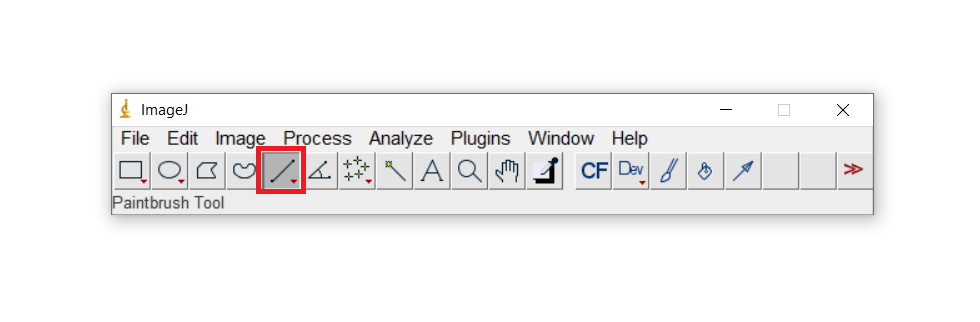
\includegraphics[width=0.7\textwidth]{galactic-center/line_tool.png}
	\caption {Top panel of ImageJ software with straight line tool highlighted.}
	\label{gc:fig:linetool}
\end{figure}

\begin{figure}
	\centering
	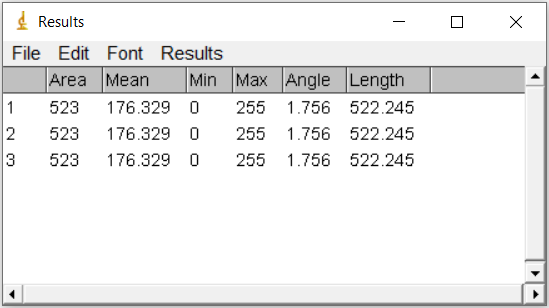
\includegraphics[width=0.7\textwidth]{galactic-center/measurement_table.png}
	\caption {Table generated by ImageJ when measuring.}
	\label{gc:fig:measurement}
\end{figure}

\begin{steps}
	\item First, note the white arrow located on the left-hand side of the image. This indicates the angular scale of the image. In the top menu bar, click on the straight line icon (see  figure \ref{gc:fig:linetool}). Now click one end of the arrow and drag the line to the other end.
	
	\item Normally, the straight line tool measures pixel count, however, you can change the scale so that it gives you the the actual measurements according to the scale of the image. To do this, click on ``Analyze'' above the icons and select the ``set scale'' option. In the ``known distance'' box enter ``0.1''. This allows you to measure the angular separation \textit{d} of the objects in the image in arcseconds. 
	
	\item Once the scale is set, use the straight line tool (the same you used to set the scale) to draw a line along the length you want to measure and press ``m'' on the keyboard. This will generate a window with different measurements which updates each time you hit ``m'' (see figure \ref{gc:fig:measurement} for an example table). You will only be using the ``length'' (in arcseconds) measurements.% and ``angle'' (in degrees) measurements. 
	
	\item Measure the semi-major axis of both stars that you chose. Make an estimate of the uncertainty of these measurements as well. \textbf{Record the star labels and their axes measurements with uncertainties.}
	
	\item\label{gc:step:angle-to-distance} Currently your measurement is an angular separation in units of arcseconds. Kepler's Third Law deals with the physical distance, so you will need to convert the angular separation to physical distance. Convert the angular separation from arcseconds to radians. Then multiply by the distance from Earth to Sag A*, $2.47 \pm 0.05 \times 10^{20}\:$m. This gives you the distance $s$ in meters. Propagate uncertainty according to Appendix\ \ref{unc:sec:prop}. \textbf{Record your work and results.}
	
	\item Use the video to measure the period of each star's orbit. If the star you picked does not complete an entire period, develop a way to estimate the entire period. Note that the time is given in decimal years (so 2020.3 means $3/10$ of the year past the beginning of 2020). \textbf{Record your work and results.}

	\item Use Kepler's Third Law to calculate the mass of Sag A* from the orbital properties of both stars that you analyzed. Your measurement should be on the order of millions of solar masses. \textbf{Record the two calculated masses and their uncertainties.}
	
	\item Use the $t'$ statistic to determine if the calculated masses from both stars are plausibly the same value ($t' < 1$). If they are not, reconsider your methods and uncertainty analysis. \textbf{Record your work and results.}
	
	\item Make a final determination of your measurement of the mass (with uncertainty), based on your two calculated masses.

\section{Finding the size of Sag A* and testing for black hole plausibility}

	\item Using the last frame of the image, use the orbital path traced in the video which came closest to Sag A* to place an upper limit on its radius. Use the straight line tool to measure this limit in arcseconds and convert to distance in meters as in Step\ \ref{gc:step:angle-to-distance}. \textbf{Record your work and results.}

	\item Now, using the estimate you found for the mass of Sag A*, calculate its Schwarzschild radius. How does this compare to the upper limit you estimated for its radius? \textbf{Record your work and results.}
	
	\item Based on this alone, how likely do you think it is that Sag A* is a black hole? What additional evidence would you need in order to conclude this? What sources of error could be affecting your estimates? What assumptions were made in this analysis that might be incorrect? \textbf{Record your discussion and determination.}
	
\section{Checking an assumption about perspective}
	
	\item Go back and watch the video you watched at the start of the lab. This time, focus on one or two orbits and not how they change as the camera moves. How does the observed 2D shape of the orbit change? \textbf{Record your observations in the lab report}
	
	\item Once you have a good idea of how the change in perspective affects our observation of the different orbits, discuss in your group how this might lead to errors when estimating orbital parameters. Think back to the different calculations you made throughout the lab, what errors could have arisen from assuming that you were always observing orbits directly from above? If we tried using this assumption to calculate the mass of the central object in an orbit, and that assumption was false, would the mass be over- or under-estimated? \textbf{Record your answer with justification.}
\end{steps}

\section{Group functioning}

\begin{steps}
	\item Write a 100--200 word reflection on group dynamics. Address the following topics: who did what in the lab, how did you work together, how group roles functioned, what successes and challenges in group functioning did you have, and what do you want to continue doing or do differently?
\end{steps}

\subsection{Items to include in your report}

\begin{enumerate}
	\item Expression for Schwarzchild radius in terms of mass, gravitational constant, and speed of light {Step 7} \{0.25 pt\}
	
	\item Schwarzchild radii for various objects (Step 8) \{0.25 pt\}
	
	\item Observations and comparing with Kepler's first law (Step 10) \{0.25 pt\}
	
	\item Observations and comparing with Kepler's third law (Step 11) \{0.25 pt\}
	
	\item Initial impressions of video and identification of stars to measure (Steps 14--15) \{0.25 pt\}
	
	\item Measurement of semi-major axis of each star and conversion to distance (Steps 20-21) \{0.25 pt\}
	
	\item Measurement of period of each star's orbit (Step 22) \{0.25 pt\}
	
	\item Calculation of Sag A* mass using each star's orbit (Step 23) [Rubric Row G2] \{1 pt\}
	
	\item Comparison of two masses, discussion, and final judgment of Sag A*'s mass (Steps 24-25) [Rubric Row D4] \{1 pt\}.
	
	\item Measurement of upper limit on Sag A* radius and calculation of its Schwarzchild radius (Steps 26-27) \{0.25 pt\}
	
	\item Judgment on the hypothesis that Sag A* is a black hole with discussion of errors and assumptions (Step 28) [Rubric Rows C8, D8] \{2 pt\}
	
	\item Analysis of effects of angular orientation assumption (Step 29--30) [Rubric Row D9] \{1 pt\}
	
	\item A discussion of the findings of the experiment and why it's helpful (for you and/or for science) [Rubric Row F2] \{1 pt\}
	
	\item Analysis of group functioning (Step 31) \{0.5 pt\}
\end{enumerate}

%\begin{framed}
%	\textbf{Angular separation $d$ and angular orientation $\theta$}
%	
%	As stated, for this lab you will be focusing on the ``angular separation'' $d$ in arcseconds as well as the ``angle'' which gives the angular orientation of the line in degrees. This might be confusing as in one instance you are using an angle measurement as a distance and in the other you are using it in a more familiar manner. This measurement quirk stems from how we observe distant astronomical objects --- we can measure the angular separation directly, while the distance to the objects are more difficult to determine. In order to avoid confusion, in this lab, remember that if a formula asks for ``$\theta$'', it is asking for the angular orientation of the object in the image and if it asks for ``$d$'', it is asking for the angular separation in arcseconds. 
%\end{framed}

%\subsubsection{Measuring data for S0-2 and S0-37}
%Now you are ready to begin gathering data from the video. However, there are many different objects which you could measure and in order to avoid confusion you will be measuring two stars near Sag A* labeled S0-2 and S0-37 respectively. Using the data from these two stars and Kepler's laws, you will be able to calculate an approximate mass and size for Sag A*.  
%
%\begin{table}
%	\centering
%	\begin{tabular}{c|c|c|c|c|c}
%		frame & $d$ (arcseconds) & $s$ (m) & $\theta$ (radians) & $\Delta \theta$ (radians) & $A$ (m$^2$)
%		\\ \midrule
%		1 & & & & \cellcolor{black!25} & \cellcolor{black!25}
%		\\ \midrule
%		2 & & & & & 
%		\\ \midrule
%		3 & & & &  &
%		\\ \midrule
%		4 & & & &  &
%		\\ \midrule
%		5 & & & & &
%		\\ \midrule
%		6 & & & & &
%		\\ \midrule
%		7 & & & & &
%		\\ \midrule
%		8 & & & & &
%		\\ \midrule
%		9 & & & & &
%		\\ \bottomrule
%	\end{tabular}
%	\caption{Data table for one stellar orbit. Note that you will not have any calculations for the gray cells for frame 1, since there is no previous frame to compare to.}\label{gc:tab:orbits}
%\end{table}		
%\begin{steps}
%	\item In a spreadsheet program, make two separate tables following the format from Table \ref{gc:tab:orbits}, one for each star you will track.
%	
%	\item Load the first frame in ImageJ and locate the stars labeled S0-2 and S0-37. Using the straight line tool, measure the angular separation $d$ from Sag A* to both stars, as well as the angle $\theta$.  \textbf{Record these measurements in the respective table for each star.}
%	
%	\item Convert the angular separation from arcseconds to radians. Then, to get the physical distance between them, multiply by the distance from us to them, $2.47 \pm 0.05 \times 10^{20}\:$m. This gives you the distance $s$ in meters. \textbf{Record this in the table under the $s$ column.}
%	
%	\item Convert the angle $\theta$ from degrees to radians.
%	
%	\item After you have calculated the distance $s$ in meters and the angle $\theta$ in radians for all frames, calculate the area swept out the stars using
%	\begin{equation}
%		A_i = \pi \left( \frac{s_{i} + s_{i-1}}{2} \right)^2 \left( \frac{\theta_{i}-\theta_{i-1}}{2\pi} \right) \,,
%	\end{equation}
%	where \textit{i} and $i-1$ are a frame and the frame before it respectively. This equation gives the area by taking the area of a circle with radius given by the average distance from the object to the central mass, then multiplies it by the fraction of circle covered between the two points. Find the area covered each frame (except for the first) and \textbf{record these in the table.}
%	
%	\item Based on your measurements and calculations, does Kepler's second law hold? Are there any discrepancies? What factors could account for these discrepancies? \textbf{Record your answers.}
%	
%	\item Now, starting from the beginning of the video, estimate the orbital period for both S0-2 and S0-37. Use the time-stamp in the top-left corner (YEAR/MONTH). Convert your estimate into seconds, and estimate your uncertainty. \textit{Hint: S0-37 does not complete a full orbit. However, we know that its orbit is circular. Using this fact, estimate S0-37's period.} \textbf{Record your work and estimation.}
%
%	\item After estimating the orbital periods, for S0-2 and S0-37, use the equation from Kepler's third law to calculate the mass of Sag A*, using the final measurement for the distance $s$ as the value for the semi-major axis $a$. How does this compare to the mass $M_\mathrm{bh} = 4.0 \pm 0.05 \times 10^6\:\textrm{M}_\textrm{\astrosun}$ as measured by Boehle \textit{et al.} in 2016?
%	
%	\item How different was your estimate from Boehle \textit{et al.}'s mass? Use the $t'$ statistic to compare. What factors could have contributed to this difference? What assumptions did you have to make when estimating the period? How did you account for the effects of inclination? Why can we use Kepler's third law here? \textbf{Write down your answers in the lab report.}
%	
%	\item Using the last frame of the image, use the orbital path traced in the video which came closest to Sag A* to place an upper limit on its radius. Use the straight line tool to measure this limit in arcseconds and convert to distance in meters as above.
%	
%\end{steps}

\section{Individual Homework}
Throughout the lab, you attempted to determine whether the object located at Sag A* was a black hole by constraining its size and mass through its gravitational influence on nearby stars. It is possible to place further constraints on its size by measuring the time between fluctuations in the electromagnetic signal emitted by the object. Although Sag A* does not emit any significant light in the optical range of the spectrum, it does emit strong X-ray and radio frequencies. Moreover, the signals in these frequencies flare up on average once a day for short periods of time. However, since the speed of light is finite, light from one side of the object facing away from us will take more time to reach us than light from the side facing us. We can take advantage of this time difference to estimate how big an object is. 

\begin{enumerate}
	\item Use figure \ref{gc:fig:light-curve} to find an upper bound on the size of Sag A* in this way. How does this compare to the size you calculated during lab? 
\end{enumerate}

\begin{figure}
	\centering
	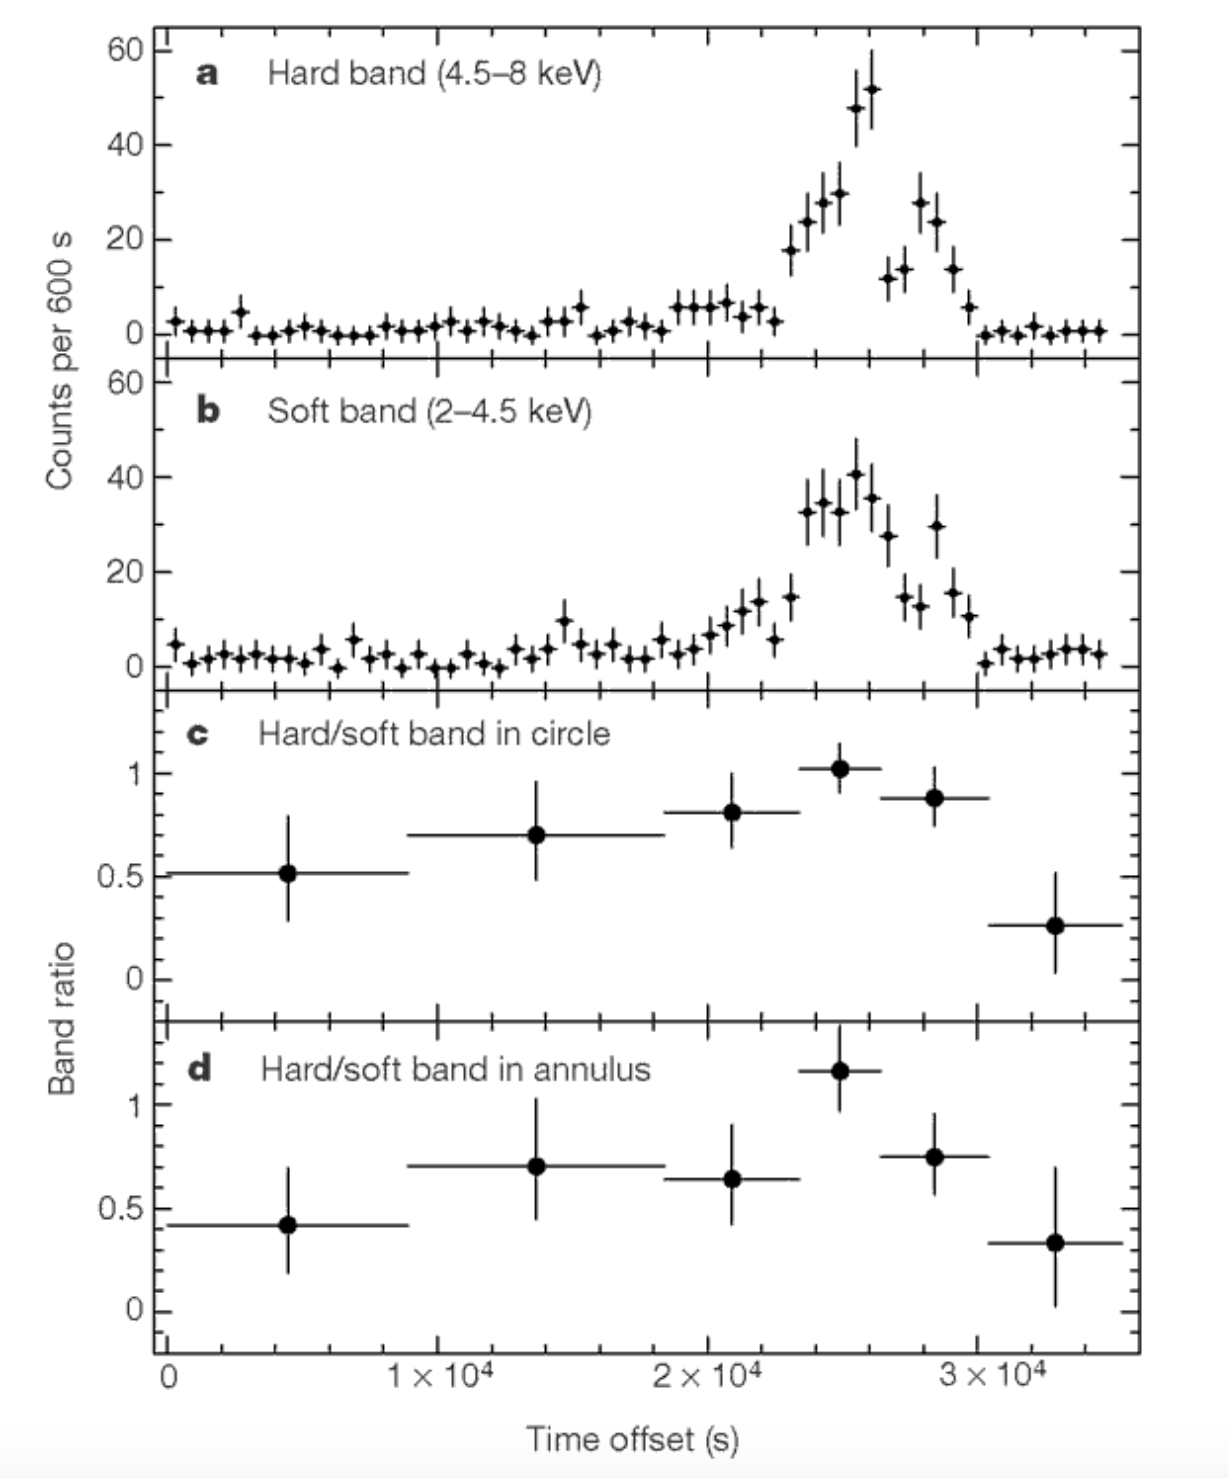
\includegraphics[width=0.7\textwidth]{galactic-center/sag-a-light-curve.png}
	\caption{Sag A* light curve, showing significant flaring on the timescale of a day.
		(from \url{https://heasarc.gsfc.nasa.gov/docs/objects/galaxies/sag-a star.html})}\label{gc:fig:light-curve}
\end{figure}

